\documentclass[a4paper, twoside]{report}

%% Language and font encodings
\usepackage[english]{babel}
\usepackage[utf8x]{inputenc}
\usepackage[T1]{fontenc}

%% Sets page size and margins
\usepackage[a4paper,top=3cm,bottom=2cm,left=3cm,right=3cm,marginparwidth=1.75cm]{geometry}

\usepackage[hyphens,spaces,obeyspaces]{url}
%% Useful packages
\usepackage{amsmath}
\usepackage{graphicx}
\usepackage[colorinlistoftodos]{todonotes}
\usepackage[colorlinks=true, allcolors=blue]{hyperref}
\usepackage[numbers]{natbib}
\usepackage{indentfirst}
\usepackage{amsmath}
\usepackage{amsthm}
\usepackage{amssymb}
\usepackage{scrextend}
\usepackage{graphicx}
\usepackage{float}
\usepackage[ruled,vlined]{algorithm2e}
\usepackage[justification=centering]{caption}% or e.g. [format=hang]
\usepackage{tikz}
\usetikzlibrary{calc,trees,positioning,arrows,chains,shapes.geometric,%
    decorations.pathreplacing,decorations.pathmorphing,shapes,%
    matrix,shapes.symbols}

\tikzset{
>=stealth',
  punktchain/.style={
    rectangle, 
    rounded corners, 
    % fill=black!10,
    draw=black, very thick,
    text width=10em, 
    minimum height=3em, 
    text centered, 
    on chain},
  line/.style={draw, thick, <-},
  element/.style={
    tape,
    top color=white,
    bottom color=blue!50!black!60!,
    minimum width=8em,
    draw=blue!40!black!90, very thick,
    text width=10em, 
    minimum height=3.5em, 
    text centered, 
    on chain},
  every join/.style={->, thick,shorten >=1pt},
  decoration={brace},
  tuborg/.style={decorate},
  tubnode/.style={midway, right=2pt},
}

\newcommand{\vpi}[1]{$V^{\pi}(#1)$}
\newcommand{\vpidash}[1]{$V^{\pi'}(#1)$}
\newcommand{\voptimal}[1]{$V^{*}(#1)$}

\newcommand{\qpi}[1]{$Q^{\pi}(#1)$}
\newcommand{\qoptimal}[1]{$Q^{*}(#1)$}
\newcommand{\qpidash}[1]{$Q^{\pi'}(#1)$}

\DeclareRobustCommand{\bbone}{\text{\usefont{U}{bbold}{m}{n}1}}
\DeclareMathOperator{\EX}{\mathbb{E}}% expected value

\title{Resource management for LoRaWAN devices with reinforcement learning with NOMA}
\author{Leon Khalmetov}
% Update supervisor and other title stuff in title/title.tex

\begin{document}
\begin{titlepage}

\newcommand{\HRule}{\rule{\linewidth}{0.5mm}} % Defines a new command for the horizontal lines, change thickness here

%----------------------------------------------------------------------------------------
%	LOGO SECTION
%----------------------------------------------------------------------------------------


\includegraphics[width=8cm]{title/logo.eps}\\[1cm] % Include a department/university logo - this will require the graphicx package
 
%----------------------------------------------------------------------------------------

\center % Center everything on the page

%----------------------------------------------------------------------------------------
%	HEADING SECTIONS
%----------------------------------------------------------------------------------------

\textsc{\LARGE MEng Individual Project}\\[1.5cm] % Name of your university/college
\textsc{\Large Imperial College London}\\[0.5cm] % Major heading such as course name
\textsc{\large Department of Computing}\\[0.5cm] % Minor heading such as course title

%----------------------------------------------------------------------------------------
%	TITLE SECTION
%----------------------------------------------------------------------------------------
\makeatletter
\HRule \\[0.4cm]
{ \huge \bfseries \@title}\\[0.4cm] % Title of your document
\HRule \\[1.5cm]
 
%----------------------------------------------------------------------------------------
%	AUTHOR SECTION
%----------------------------------------------------------------------------------------

\begin{minipage}{0.4\textwidth}
\begin{flushleft} \large
\emph{Author:}\\
\@author % Your name
\end{flushleft}
\end{minipage}
~
\begin{minipage}{0.4\textwidth}
\begin{flushright} \large
\emph{Supervisor:} \\
McCann, Julie \\[1.2em] % Supervisor's Name
\emph{Second Marker:} \\
Maffeis, Sergio 
\end{flushright}
\end{minipage}\\[2cm]
\makeatother

% If you don't want a supervisor, uncomment the two lines below and remove the section above
%\Large \emph{Author:}\\
%John \textsc{Smith}\\[3cm] % Your name

%----------------------------------------------------------------------------------------
%	DATE SECTION
%----------------------------------------------------------------------------------------

{\large \today}\\[2cm] % Date, change the \today to a set date if you want to be precise

\vfill % Fill the rest of the page with whitespace

\end{titlepage}

% \begin{abstract}
% Your abstract goes here
% \end{abstract}

% \renewcommand{\abstractname}{Acknowledgements}
% \begin{abstract}
% Thanks mum!
% \end{abstract}

\tableofcontents
% \listoffigures
% \listoftables

\chapter{Introduction}

% According to Cisco IBSG the Internet of Things was born somwhere between 2008 and 2009 at “the point in time when more ‘things or objects’ were connected to the Internet than people”\footnote{https://www.cisco.com/c/dam/en_us/about/ac79/docs/innov/IoT_IBSG_0411FINAL.pdf}\footnote{https://www.cisco.com/web/offer/emear/29676/tnc2013/documents/IoEandOlympics.pdf}. Furthermore in 2020 for the first time there are more "IoT connections" (e.g., connected cars, smart home devices, connected industrial equipment) than there are "non IoT connections" (smartphones, laptops, and computers) according to the latest report by  IOT Analytics\footnote{https://iot-analytics.com/state-of-the-iot-2020-12-billion-iot-connections-surpassing-non-iot-for-the-first-time/}. The paradigm is becoming evermore relevant and with the global pandemic it's focus would expand from using smart sensors for saving energy to social distancing in the workplace and tracking technologies to fight COVID-19\footnote{https://www.iotworldtoday.com/2021/01/07/iot-trends-2021-a-focus-on-fundamentals-not-nice-to-haves/}.\\

% IoT devices typically operate on strict energy constraints having limited power (battery or solar) and communicating over long distances. In contrast to the exisiting 4th or 5th generation communication technologies, the high data rate is typically traded for longer communication ranges. This can be achieved with low-power wide-area networks (LPWAN). Among the various LPWAN technologies this project will investigate into the LoRa (Long Range) protocol originally developed by Cycle of Grenoble France and acquired by Semtech in 2012 \footnote{https://www.forbes.com/companies/semtech/?sh=36d0faf84e3e}.\\

% The main focus of this project will be to look into ways to apply different Reinforcement learning techniques to develop resource management techniques for IoT devices to maximize efficiency, reliability and coverage of LoRaWAN protocol for LPWAN with a focus on nonorthogonal multiple access (NOMA) radio techniques. \\

% In chapter 2 we will look into basic concepts of LoRA. In chapter 3 we will review a simulation framework to be used for conducting experiments. In chapter 4 we will look into Reinforcement Learning techniques that could potentially be applied in this case. 


\chapter{LoRa}

LoRa stands for \textbf{Lo}ng \textbf{Ra}nge. It is a transmission standard that aims at achieving long range reach with low power consumption, most commonly used by the Internet of Things devices. LoRa technology was first developed by Cycleo from Grenoble, France around 2010 with first prototypes implementing point-to-point communication for walkie-talkie and metering applications \cite{trinity_panel}. Later in 2012 the Cycleo team was aquired by Semtech, and released the chips for LoRa end devices and gateways \cite{origins}. \\

The open non profit organisation LoRa Alliance emerged in 2015\cite{alliance}. 
It is an association of companies with Semtech being one of
its founding members \cite{alliance_founder} backing up the LoRaWAN protocol, insuring its
global presence and acceptance. The total number of members of the alliance has surpassed 500 in 2017 \cite{500_members}. Among the notable members are Cisco, Amazon and Alibaba \cite{alliance_members}.

\subsection{LoRa Spread Spectrum (Chirp Spread Spectrum)}

% There are 2 main modulation techniques used for radio broadcasting: AM, i.e amplitude modulation and FM, i.e. frequency modulation whereby either amplitude or frequency are modulated. \\

Chird Spread Spectrum is a modulation scheme, whereby the frequency of a signal is changing linearly in time \cite{ieee_2007} as shown on the figure below \ref{fig:slope}. Such sweeps in frequency are called chirps. CSS is a modulation technique that has been around since 1940s
\cite{semtech_spec} with applications in naval and air military and also observed in fauna \cite{origins}.\\

In regards to LoRa CSS signals are bounded by the specified symbol duration and bandwidth. Symbol duration $t_s$ determines the time period over which the frequency sweep occurs and bandwidth defines the sweep range between starting frequency $f_{min}$ and $f_{max}$ on the diagram, i.e. bandwidth = $f_{max} - f_{min}$. Moreover the sweep can start at any frequency $f_0$ (determined by the number of input bits) between $f_{min}$ and $f_{max}$ and this means that a signal can be represented by multiple chirps as demonstrated in the
diagram below. So if the sweep reaches $f_{max}$ before $t_s$ it 
continues from $f_{min}$ until time = $t_s$. Thus if $f_0 = f_{min}$
the signal will end at $f_{max}$ exactly without breaking up. 

\begin{figure}[H]
  \centering
  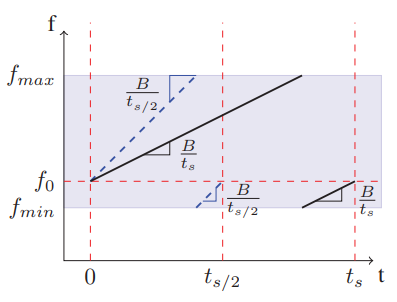
\includegraphics[scale=0.5]{figures/slope.PNG}
  \caption{Graphical representation of the frequency in time for 2 spreading factors. Source: \cite{slope_diagram}}
  \label{fig:slope}
\end{figure}

% What makes CSS different from other Spread Spectrum techniques (despite some claiming it to be a subtype of DSSS \cite{orthogonality_description}) is the fact that it is resistant to multi-path fading and Doppler effect while having relatively moderate transmission power demands \cite{semtech_spec}. \\

% Spreading factor determines the number of bits to be encoded in a signal \cite{sf}

% LoRa employs six spreading factors from 7 to 12 to provide orthogonality in data transmission (collision-free) occurring on the same frequency.  SF determines the chirp rate — change in frequency with respect to time which is the slope on \ref{fig:slope}{}

% An advantage of LoRa spread spectrum is that timing and frequency offsets between transmitter and receiver are equivalent, greatly reducing the complexity of the receiver design. \cite{semtech_spec}  

\subsection{Spreading factors}

According to the Semtech specification \cite{semtech_spec} symbol duration $t_s$ can be calculated using this formula:
\begin{align}
    T_S = \frac{2^{SF}}{B} 
\end{align}

Where $SF$ stands for spreading factor. Thus looking at figure \ref{fig:slope} SF determines the slope of the chirps, i.e. $\frac{B}{T_s}$ and the number of bits in the encoded information \cite{sf_article}, i.e. $f_0$.\\

According to the spec \cite{semtech_spec} LoRa employs 6 spreading factors from 7 to 12. Spreading factors allow different signals to be transmitted over the same channel at the same time. As the specification claims it is possible due to the orthogonality of CSS signals of different spreading factors to each other \cite{semtech_spec}.
Despite the claim of the orthogonality feature of spreading factors in CSS signals, it has been shown to be quasi-orthogonal and the decoding of signal at the receiver can be disrupted under certain conditions for example if the power of the interfering signal is stronger than the one to decode \cite{imperfect_1}.

\section{LoRaWAN}

On top of the physical layer there needs to be a protocol. And such is the LoRaWAN layer backed by the LoRa Alliance. As the LoRa Alliance itself states on its website \cite{lora_alliance_about_lorawan} LoRaWAN is a network protocol of communication between Internet of Things devices.

\subsection{Network Topology}

The LoRaWAN standard is based on a star topology.
Multiple end devices (nodes) communicate with a gateway (base station) and multiple gateways communicate with the main network server as demonstrated in the figure \ref{fig:star}. Here gateway acts as an agent between the nodes and the internet, translating Radio Frequency messages into Internet Protocol packets and vice-versa \cite{lora_alliance_about_lorawan}.
One gateway can typically cover a range of hunderds of meters to tens of kilometers with up to millions of end devices \cite{doppler}.

\begin{figure}[h!]
  \centering
  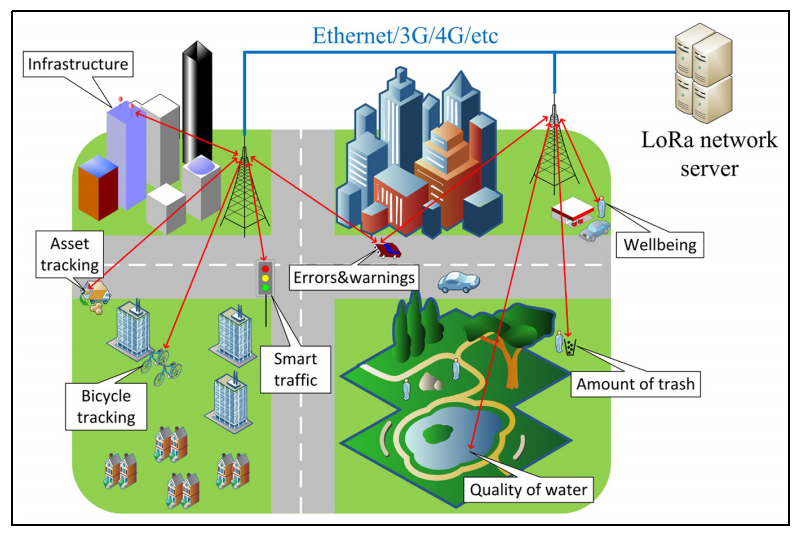
\includegraphics[scale=0.4]{figures/start-topology.PNG}
  \caption{LoRaWAN nodes and gateways connected to a LoRa server Source: \cite{doppler}}
  \label{fig:star}
\end{figure}

\subsection{Multiple Access Control (MAC) scheme}

LoRaWAN implements ALOHA protocol where any device can wake up and transmit a message regardless of time. We are concerned with the messages between a LoRaWAN device and a gateway (base station). Requests from a node to a gateway are called uplink messages, and the responses are called downlink messages.  
The communication scheme has an uplink-centric design and 
LoRaWAN mandates this design for all devices implementing the protocol \cite{simulator}. In the figure \ref{fig:class A} one can see the typical cycle a node goes through while communicating with a particular gateway. The receive windows are allocated periods of time when the node is expecting 
a downlink response that should follow its uplink request.

\begin{figure}[h!]
  \centering
  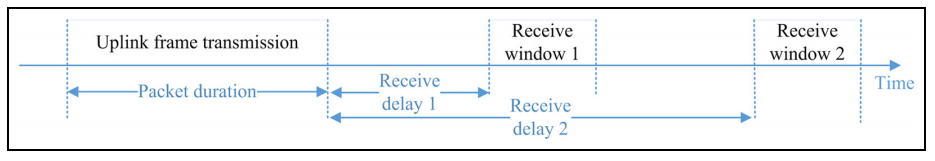
\includegraphics[scale=0.5]{figures/class A.PNG}
  \caption{Class A type LoRaWAN device scheduling of receive slots for downlink messages. Source: \cite{doppler}}
  \label{fig:class A}
\end{figure}

There are 3 different device types based on the way to schedule the receive window slots for downlink communication: class A, B and C. Support for class A (demonstrated in the figure \ref{fig:class A} above) is compulsory with B and C being extensions to it. Class A devices schedule 2 receive windows following an uplink transmission, class B devices open receive windows periodically and class C devices listen for downlink messages continuously unless they are transmitting \cite{lora_alliance_spec}. 

\subsection{Duty cycle}
For each band LoRaWAN devices operate in, they need to comply with the industrial, scientific and medical (ISM) regulations often set by the local government \cite{duty_cycle}. These include the duty cycle limitation that determines amount of time a device can be active within a bandwidth. For example in Europe the duty cycle standards are set by the 
European Telecommunications Standards Institute (ETSI) \cite{about_etsi}.\\
% "the recognized regional standards body dealing with telecommunications, broadcasting and other electronic communications networks and services.", as their website   states.\\ 

What duty cycle basically controls is the fraction of time a device can be active on a particular sub-band (potentially on multiple channels) \cite{duty_cycle}. For example if the channel in 
question is used for 1 time unit for every 10 time units,
the device using it has a duty cycle of 10\%. If we take into account multiple channels (within one sub-band), then we count in the total fraction of time these channels are being used by the device \cite{duty_cycle}. [INFO ABOUT section 7.2.3 of the ETSI EN300.220 standard]

\section{NOMA}
 
 Non-Orhogonal Multiple Access (NOMA) scheme is a relatively new concept first introduced in this publication \cite{noma_original} in 2013. As opposed to orthogonal
frequency division multiplexing (OFDM), NOMA decodes multiple incoming signals, occupying the same time 
or frequency resources, utilizing the power or code domain \cite{noma_imperial}. [DIAGRAM FROM TUTORIAL]. In the power domain implementation of NOMA the decoding is achieved via successive interference cancellation (SIC) based on the different power levels of the incoming signals \cite{noma_imperial} \cite{noma_original}. \\

Basically what happens is that the incoming signals are decoded at the receiver in the order of decreasing channel gain, so the  strongest one is decoded first and the weakest is decoded last. Signals are decoded in that order so as to minimize the interference different signals experience \cite{noma_imperial}. After the strongest current signal is decoded, the total interference for other signals (to be decoded yet) is reduced by its largest component.\\

Despite the original paper \cite{noma_original} focusing on the downlink NOMA
implementation (i.e. end-device/node being the receiver in question), we are interested in the uplink communications and thus the workings of NOMA at the gateway. 
  
%  As the name NOMA suggests, it it does not utilizes the orthogonality of 
%  , but instead decodes multiple incoming signals based on the 
 
 
\section{LoRa Simulation Framework}

In order to simulate a LoRaWAN network I have decided to pick one described in this paper \cite{simulator}. The developers of the paper have closely followed guidelines from The Things Network (TTN)\footnote{https://www.thethingsnetwork.org/}, which is an open community of volunteers that took on an initiative to contruct and maintain LoRaWAN stations around the world to reach its global coverage. On their website they also provide tutorials and guides to help people deploy LoRaWAN gateways and nodes. The simulation code is published in github \cite{simulator_github}. The developers have decided to simulate the LoRaWAN network via the \texttt{SimPy} which is a Python discrete-event simulation framework library\cite{simpy}. The simulation is mainly driven through continuous yielding of appropriate generator functions. A potential improvement to the code would be introduction of some sort of parallelisation.

\subsection{Architecture}

The simulation is based on the LoRaWAN architecture of star-toppology network with mutiple nodes connected to a single gateway as already described above and in the figure \ref{fig:star}. The simulation supports only one gateway, so among other improvements would be introduction of multiple gateways in the simulated area. \\

In the following figure \ref{fig:architecture} is the scheme describing relations between the most relevant simulation python classes (along with their names).

\begin{figure}[h!]
  \centering
  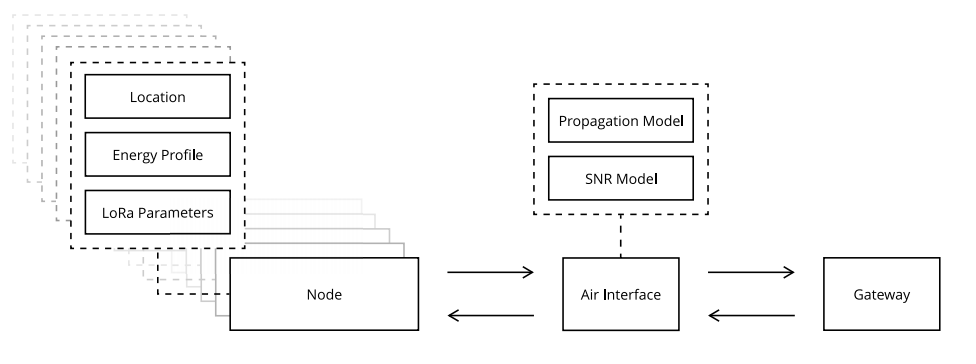
\includegraphics[scale=0.5]{figures/architecture.PNG}
  \caption{Interaction between python classes: \cite{simulator}}
  \label{fig:architecture}
\end{figure}

\subsection{Nodes}

As can be seen from the figure \ref{fig:architecture} the \texttt{Node} object is characterized by the \texttt{Location}, \texttt{Energy Profile} and \texttt{LoRa Parameters} objects (among others) passed to its constructor during initialization as parameters.\\

\texttt{Location} as its name suggests, simply holds the coordinates for a particular Node. The simulation assumes a rectangular cell, and the particular node location is typically randomly selected within the bounds of that rectangle. \\

\texttt{Energy Profile} holds information about the different power states and their duration in the execution loop of communication between a node and its respective gateway (sketched above in \ref{fig:class A}). The energy profile used in the original paper \cite{simulator}, as the authors stated was motivated by the energy consumption analysis of another project — LoRaWAN implementation for the EFM32 Happy Gecko develop board \cite{energy_profile}. The energy profile used is displayed in the figure below:

\begin{figure}[h!]
  \centering
  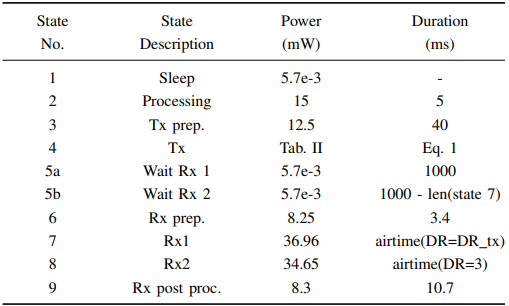
\includegraphics[scale=0.7]{figures/energy_profile.PNG}
  \caption{Energy Profile devised from \cite{energy_profile}. Source: \cite{simulator}}
  \label{fig:energy_profile}
\end{figure}\\

The effect of implementing this energy profile can be seen in the figure \ref{fig:power_states} below; it displays, how the power states of a node develop in time:

\begin{figure}[h!]
  \centering
  \hspace*{-1cm}  
  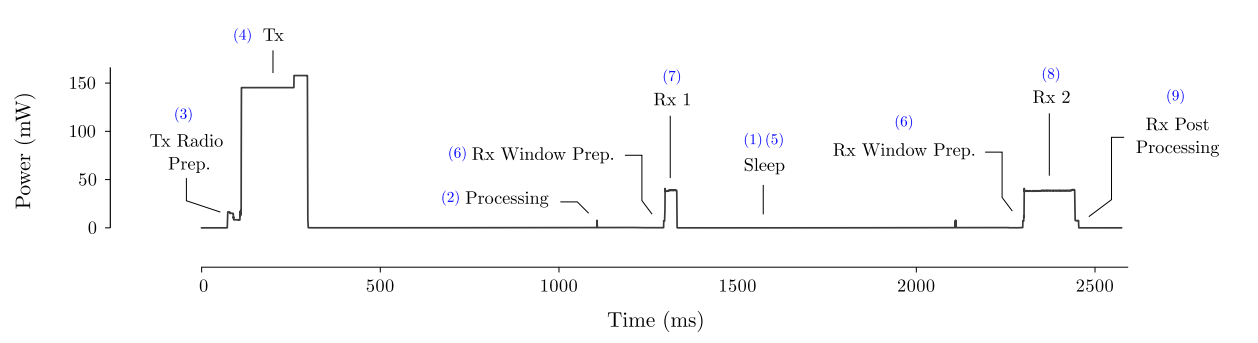
\includegraphics[scale=0.5]{figures/class A 2.PNG}
  \caption{Power states of a LoRa node simulated in \cite{simulator}}
  \label{fig:power_states}
\end{figure}\\

\texttt{LoRa Parameters} object holds information about the configuration of the uplink packets that the Node is going to send, such as its spreading factor, frequency (channel) and transmission power. These are the factors that play a crucial role in the resulting energy consumption at the node \cite{simulator}.

\subsection{AirInterface}

\texttt{AirInterface} is the object via which \texttt{Node} and \texttt{Gateway} communicate. It processes the packets "in the air" and determines their airtime as well as simulating collisions between packets. It also defined by the \texttt{Propagation Model}.\\

\texttt{Propagation Model} calculates the path loss 
of a signal traveling in the channel through the air.
the formula is defined in the original paper \cite{simulator} :
\begin{align}
    PL(d) = PL(d_0) + 10n\times log\frac{d}{d_0} + X_{\sigma} [dB] \label{eq:propagation_model}
\end{align}

Where the following parameters are used. These measurements were taken by the authors \cite{simulator} from measurements reported here \cite{propagation_model_parameters}):
\begin{align*}
     d_0 & = 1000 \text{m}\\
     PL(d_0) & = 128.95 \text{dB}\\
     X_{\sigma} & = 7.8 \text{dB}\\
     n & = 2.32\\
\end{align*}

Collision model is not implemented as a separate object but through a collection of functions in \texttt{Air Interface}. The model implementation is motivated by the authors \cite{simulator} by the findings from another paper \cite{collision_conditions}, that looks at how reception overlap, carrier frequency, spreading factor and power can create conditions for a packet collision. The authors \cite{simulator} also assume that signals with different spreading factors are practically orthogonal and can be demodulated without colliding.\\

\texttt{SNR} model was implemented in the original framework to
calculate the Signal-to-Noise ratio values for the packets in the air, but in my implementation I'll use another metric 
described later in my modifications.

\subsection{Gateway}

\texttt{Gateway} object is responsible for receiving 
the uplink packets from the \texttt{Air Interface}. In order for a packet to come through it must not collide and have  a signal strength above that of gateway's specified sensitivity. In the original simulator \cite{simulator} \texttt{Gateway} is also responsible for executing the ADR algorithm. ADR is the algorithm, devised to minmize the energy consumption at nodes, operating mainly by estimating the appropriate TP and SF values for each uplink packet and sending them to the respective node (that sent the packet) via a downlink frame \cite{simulator}. The node that uses these values until a next update from the gateway. In the original simulator these values are calculated based on the SNR values of the received frames. 
[INPUT DETAILS ON ADR and ADR itself maybe] \\

In this project, however we are not going to implement any form of ADR and instead apply reinforcement learning tecnhiques to 
decide on appropriate \texttt{LoRa Parameters} values for uplink frames.


% Due to the SF orthogonality assumption, the gateway can simultaneously receive up to 8 different packets on separate channels. [FALSE???]

\chapter{Reinforcement Learning} 

Reinforcement Learning has recently seen a rise in popularity after a few successful case studies such as the success of DeepMind in 2016 after AlphaGo beat the Korean 9-dan professional Go player \cite{alpha_go_lee_sedol} and after more recently OpenAI beat a team of professionals in a Dota 2 match \cite{dota}.\\

Reinforcement Learning (RL) typically focuses on the problems of agents within some environment. The agents try to learn optimal behaviour within the environment, with the goal of maximizing some sort of reward (e.g. AlphaGo playing Go, trying to maximize it's win probability \cite{alpha_go_lee_sedol}). The policy of that agent, i.e. how it decides to act under certain conditions (e.g. coordinates on a map, temperature, board game position) is the component, not specified by the programmer but instead learnt by the agent via trial-and-error interactions with the environment over the learning period \cite{sutton_barto}. Thus RL often reduces to a problem of learning the optimal policy in the context of a particular application.\\

This closed loop can be demonstrated as in the figure \ref{fig:closed_loop} below, where an agent subject to state $S_{t}$
and reward $R_{t}$ takes an action $A_{t}$ which leads to a new
state $S_{t+1}$ and a new reward $R_{t+1}$:

\begin{figure}[h!]
  \centering
%   \hspace*{-1cm}  
  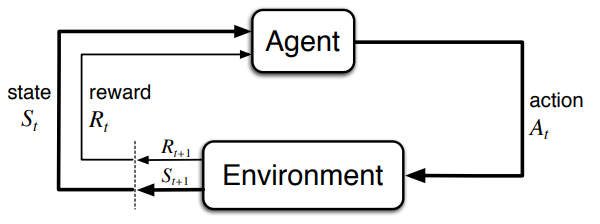
\includegraphics[scale=0.7]{figures/closed_loop.PNG}
  \caption{Closed-loop of reinforcement learning. Source: \cite{sutton_barto}}
  \label{fig:closed_loop}
\end{figure}\\  

% \section{Terminology and symbols}
% Here I'll explain the main bulk of terminology specific to reinforcement learning that we'll need for the rest of this chapter.\\

% Rewards, Action, States, Policy, Value function [DO LATER]
 
\section{Markov Decision Process}

In this section I'll touch upon the basic mathematics of evaluating the environment around the learning agent and the 
main concepts that will be used later in the 
Deep Reinforcement Learning model section.

Markov Decision Process is a Markov Chain based decision making
tool defined by state space $S$, action space $A$, transition 
probability matrix $P^{a}_{ss'}$, reward 
% $P^{a}_{ss'} = p(s_{t+1}| s_t, a_t)$
function $R$ and decision policy $\pi$ \cite{lecture_mdp}. In 
the subsections below I will explain what each of these is.

\subsection{Markov chain}
Markov Chain is essentially a way to model stochastic
processes with particular properties. As the name suggests it is a chain of states that describes the process we are modeling. Using an exmaple from this article \cite{markov_chain_article}, if we
are to model weather at a particular region on a daily basis,
we could have 2 states: Sunny and Rainy. Now what interests us
are the transitions between these 2 states. We could model
them as a simple random process such that the probability of
it being Sunny after being Rainy was 0.5 and the probability
of it being Rainy after being Sunny was 0.1. Furthermore if we
assume the \textbf{memorylessness} property of this model i.e.
that the weather tomorrow is \textbf{independent} of the
weather yesterday and only depends on the weather today then
we could effectively derive the other 2 missing probabilites
for the weather staying Sunny (1 - 0.1 = 0.9) or Rainy (1 -
0.5 = 0.5) for 2 days in a row \cite{markov_chain_article}. This example is demonstrated in figure \ref{fig:weather}.

\begin{figure}[H]
  \centering
%   \hspace*{-1cm}  
  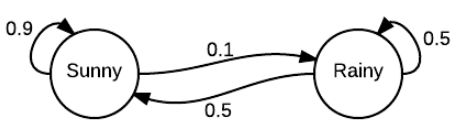
\includegraphics[scale=0.7]{figures/markov_weather.PNG}
  \caption{Markov chain for weather forecasting. Source: \cite{markov_chain_article}}
  \label{fig:weather}
\end{figure}

Thus we can describe a Markov process through a set of states S and a probability transition matrix P satisfying the \textbf{Markov property} (memorylessness) \cite{markov_chain_article}:
\begin{align}
    P_{ss'} = P[S_{t+1} = s' | S_{t} = s]\\
    \sum_{s' \in S} P_{ss'} = 1
\end{align}

\subsection{Policy}
As mentioned above an agent within an environment is capable of taking an action a. The sequence of actions taken under 
various conditions is defined by the agent's policy.
A policy $\pi$ is typically a conditional probability distribution that allows an agent to choose its next action in a defined state at a defined time \cite{lecture_lets_go_markov}:
\begin{align}
    \pi_t(a, s) = P[A_t = a | S_t = s]
\end{align}

\subsection{Reward function}
The reward function $R$ maps transitions between states within a
Markov Decision Process to their respective reward values.
$R_{ss'}^{a}$ is the immediate reward an agent receives if starting from state $s$ it takes an action $a$ and transitions to state $s'$.\\

We can also define the total return value $R_t$ which is the estimated sum of all immediate rewards $r$ starting from time-step t:
\begin{align}
    R_t = r_{t+1} + \gamma r_{t+2} + \gamma ^2 r_{t+3} + ... = \sum^{\infty}_{k=0}\gamma^{k}r_{t+k+1} \label{eq:return}
\end{align}

Where $\gamma$ is the discount factor such that $\gamma \in [0, 1]$ \cite{lecture_lets_go_markov}. The discount factor allows the agent to put different weight on immediate and distant rewards, with smaller $\gamma$ being more concerned with immediate results and larger $\gamma$ looking far into the future. 

% \begin{align}
%     R_{ss'}^{a} = E[r_{t+1} | S_{t} = s, A_{t} = a] \label{eq:return_matrix}
% \end{align}

% This is the reward that the agent leaving state s receives upon transitioning at timestep $t+1$.\\

% [WHY DISCOUNTING IS A GOOD IDEA SLIDE 56 https://materials.doc.ic.ac.uk/view/2021/70028/Course\%20Material/7]
\subsection{State Value Function}
State Value Function $V$ is the estimate of the total return one expects to retrieve starting from a state $s$ at time $t$ in the context of a Markov Decision Process with a policy $\pi$ \cite{lecture_lets_go_markov}. If we expand the expectation term:
% \begin{align}
%      
% \end{align}

% If we now account for an MDP policy $\pi$ and expand the original definition \ref{eq:value_function_def} \cite{lecture_mdp}:
\begin{align}
    V^{\pi}(s) &= \EX_{\pi}[R_{t} | S_t = s]  \label{eq:value_function_definition} \\
    &= \EX[\sum^{\infty}_{k=0} \gamma^k r_{t+k+1} | S_t = s] \nonumber \\
    &= \EX[r_{t+1} + \gamma \sum^{\infty}_{k=0} \gamma^k r_{t+k+2} | S_t = s] \nonumber \\
    &= \EX[r_{t+1} + \gamma R_{t+1} | S_t = s] & \text{definition \ref{eq:return}} \nonumber \\
    &= \EX[r_{t+1} + \gamma \EX[R_{t+1} | S_t = s] | S_t = s] & \text{Adam's Law} \nonumber \\
    &= \EX[r_{t+1} + \gamma V^{\pi}(S_{t+1}) | S_t = s] & \text{definition \ref{eq:value_function_definition}} \nonumber \\
    &= \EX[r_{t+1} + \gamma V^{\pi}(s') | S_t = s] \nonumber \\
    &= \sum_{a \in A} \pi(s, a) \sum_{s' \in S} P^{a}_{ss'} (R^{a}_{ss'} + \gamma V^{\pi}(s')) &\text{expanding $\EX$} \label{eq:mdp_value_function_expansion}
    \label{eq:value_function_def}
\end{align}

where 
\begin{align*}
    \pi(a, s) &= P[a|s] &\text{policy i.e. probability of taking action $a$}\\
    P^{a}_{ss'} &= P[s' | s, a] &\text{state-action transition probability}\\
    R^{a}_{ss'} &= r(s, a, s') &\text{immediate reward function}
\end{align*}

% Converting the last line of the above derivation into vector notation to account for n states (respectively n dimensions):
% \begin{align}
%     \textbf{v} = R + \gamma P \textbf{v}
% \end{align}

% A direct solution to this would be 
% \begin{align}
%     \textbf{v} = (\bbone - \gamma P)^{-1}R
% \end{align}

% Due to matrix inversion being an expensive computational operation, this kind of approach of estimating a state value function is not preferred and only works for relatively small MRPs \cite{lecture_lets_go_markov}. There are, however iterative approaches to this problem, such as Dynamic Programming, Monte-Carlo evaluation and Temporal Difference Learning.\\

Majority of all the reinforcement learning algorithms introduced in this chapter later down below will rely on this "recursive consistency" \cite{lecture_mdp} property of state value functions. 

% \subsection{Policy Evaluation}
% Now we need to find a systematic way of estimating the value
% function for a given MDP for an arbitrary policy. This process is called Policy Evaluation \cite{lecture_mdp}. The most obvious method is to apply the Bellman equation over and over again, until the value function converges as in figure \ref{fig:ipa}.
% \begin{figure}[H]
%   \centering
% %   \hspace*{-1cm}  
%   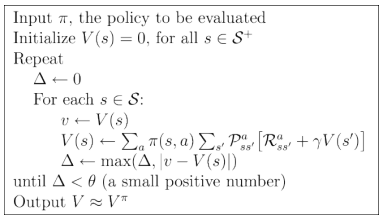
\includegraphics[scale=0.8]{figures/iterative_policy_evaluation.PNG}
%   \caption{Iterative Policy Algorithm; Source: \cite{lecture_mdp}}
%   \label{fig:ipa}
% \end{figure}

\subsection{State Action Value Function}
As an extension to the state value function we introduce the state-action value function $Q$ that evaluates the expected return for taking action $a$ at a state $s$ subject to policy $\pi$ \cite{lecture_mdp} :
\begin{align}
    Q^{\pi}(s, a) = \EX[R_t | S_t = s, A_t = a] = \EX[\sum^{\infty}_{k=0} \gamma^k r_{t+k+1} | S_t = s, A_t = a]
\end{align}

The relationship between state value and state-action value functions is as follows:
\begin{align}
    V^{\pi}(s) = \sum_{a \in A} \pi(s, a) Q^{\pi}(s, a) 
\end{align}

% An important advantage of the state-action value function over state value function is the 

\section{Learning Approaches}

In this section I'll look at different learning approaches such
as Dynamic Programming and Monte-Carlo methods and how 
these rely on agent's Model Knowledge. The final Deep Reinforcement Learning model will be based of each of these 
and will heavily rely on concepts introduced here as well. 

\subsection{Dynamic Programming}

Dynamic Programming typically refers to a set of algorithms targeted at solving problems within well-defined systems such as Markov Decision Process \cite{lecture_dp}. Typically Dynamic Programming refers to solving a problem by breaking it into smaller sub-problems and solving them recursively which 
fits in nicely with the recursive equation \ref{eq:value_function_def}.

\subsubsection{Policy Improvement}

Through the Policy Improvement Theorem \cite{lecture_dp} it is 
possible to accurately compare policies to each other and 
through that choose which State Value (or State-Action Value) Function is better for optimization purposes. Based on that it 
is possible to run a Policy Iteration Algorithm \cite{lecture_dp} which iterates
through all states of an MDP and different policies are evaluated and then improved on using the equation \ref{eq:value_function_def} derived earlier.

\subsubsection{Strengths and weaknesses}

DP introduces a useful concept: "bootstrapping" i.e. evaluating the current state value based on the neighbouring state value evaluations \cite{lecture_dp}. DP works well for moderate not resource hungry type of problems and suffers from the curse of dimensionality once the problem complexity increases. It also requires full knowledge of the Markov Decision Process which is not always available in practice.To address the weaknesses of dynamic programming Model-Free Learning comes into play.

\subsection{Monte Carlo (MC) Methods}

Monte-Carlo Methods are fundamentally different from the 
Dynamic Programming approach in that they don't require the 
full knowledge of the environment around the agent. They fall
in the category of Model-free learning algorithms \cite{lecture_mfl}. The process is based fully off of the sampled experience.  \\

The basic idea is to calculate the average return over traces of episodes, an episode being a sequence of state transitions sampled directly from the environment. A state transition includes information about original and new state, action taken and the immediate reward. One condition is that each episode must end in a terminal state. 

\subsubsection{Monte-Carlo update rule}

Like in the Policy Improvement subsection one can devise the policy evaluation algorithm based of calculating the average return over traces of episodes \cite{lecture_mfl}. 
% Here you can see that value function is approximated with an average returns of states. This is a First-Visit MC algorithm, so only the first occurence of a state is counted toward the estimate. In Every-visit MC algorithm every occurence is recorded \cite{lecture_mfl}.
% We can update the policy after every episode or after
% sampling a trace of 20 for example. the former is called online MC and the latter Batch MC.
To update the mean value for a state after each transition an incremental update from the normal definition of 'mean' can be devised as described here \cite{lecture_mfl} :
\begin{align}
    \mu_k &= \frac{1}{k}\sum^{k}_{i = 1} x_i \nonumber \\
    &... \nonumber \\
    \mu_k &= \mu_{k - 1} + \frac{1}{k} (x_k - \mu_{k - 1})
\end{align}

This is an important milestone, since the running mean can be recorded without storing traces of transitions. In the same way one can update the state value function $V(s)$ (as in Monte-Carlo it holds the average reward over episodes of experience) incrementally after each new episode (s, a, r, s'):
\begin{align}
    V(s_t) \longleftarrow V(s_t) + \frac{1}{N(s_t)}(R_t - V(s_t))
\end{align}

Moreover one can set the $N(s_t)$ value (i.e. current number of sampled transitions) to another number $n$, such that $n < N(s_t)$, by basically narrowing down the averaging operation to the last n transitions. This is in effect turns the fraction into $\alpha$ -- the rate at which old episodes are discarded \cite{lecture_mfl}:
\begin{align}
    V(s_t) \longleftarrow V(s_t) + \alpha (R_t - V(s_t)) \label{eq:mc_increment}
\end{align}

\subsection{Temporal Difference}
% We have now introduced two different approaches to finding the optimal Value function for a problem at hand: Dynamic Programming and Monte-Carlo. Dynamic programming achieves the optimal solution through "bootstrapping" i.e. estimating state values through
% neighbouring states. Monte-Carlo methods calculate the estimates through sampling directly from experience i.e. traces of episodes. \\

Temporal Difference (TD) is what combines Dynamic Programming and Monte-Carlo: like MC It does not require full model knowledge of Markov Decision Process at hand and 
learns from episodes of experience and like DP it makes use of bootstrapping \cite{lecture_mfl}.

% \begin{figure}[h!]
%   \centering
% %   \hspace*{-1cm}  
%   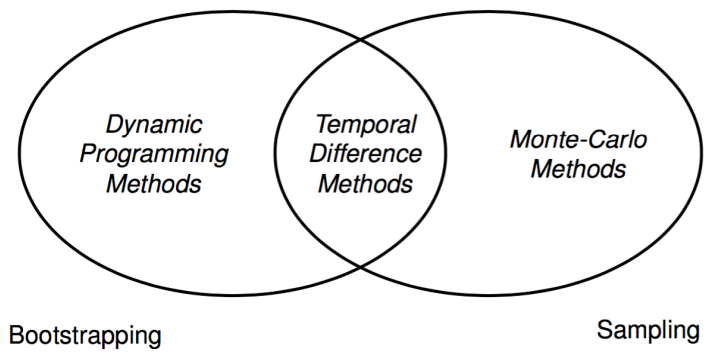
\includegraphics[scale=0.5]{figures/TD_diagrams.PNG}
%   \caption{Temporal Difference; Source: \cite{lecture_mfl}}
%   \label{fig:td}
% \end{figure}

\subsection{Update rule}
The combination of DP and MC is manifested in the value function update rule for Temporal Difference:
\begin{align}
  V(s_t) \longleftarrow V(s_t) + \alpha (r_{t+1} + \gamma V(s_{t+1}) - V(s_t)) \label{eq:td_update}
\end{align}

where:
\begin{align*}
  r_{t+1} + \gamma V(s_{t+1}) - V(s_t) &\text{ — } \text{TD error}\\
  r_{t+1} + \gamma V(s_{t+1}) &\text { — } \text{TD target}
\end{align*}

Comparing this to the update rule for MC (equation \ref{eq:mc_increment}) we can see that in addition to the actual measured reward $r_{t+1} (R_{t}$ in equation \ref{eq:mc_increment}) we add an estimate of the next state i.e. $V(s_{t+1})$. This estimation refers us back to the original estimation of the value function from equation \ref{eq:value_function_def} making TD target an estimation of the total expected return.\\

Thus in the Temporal Difference Value estimation algorithm
bootstrapping and direct sampling are combined \cite{lecture_mfl}. 

\subsection{Bias-Variance tradeoff for TD and MC}
In statistics the Bias-Variance tradeoff typically refers to 
a compelled compromise between variance and bias, i.e. either high variance and low bias or low variance and high bias. \\

We can see that $R_t = r_{t+1} + \gamma r_{t+2} + \gamma ^2 r_{t+3} + ...$ is an unbiased estimate of $V^{\pi} (s_t)$ by the definition \ref{eq:value_function_def} of the state value function itself. So if the update rule for TD was $r_{t+1} + \gamma V^{\pi}(s_{t+1})$ it would be an unbiased estimate of $V^{\pi}(s_{t})$ (given $V^{\pi}(s_{t+1})$ is the true value function). But what we actually have is an estimate of the $V^{\pi}(s_{t+1})$ — $V$ ($r_{t+1} + \gamma V(s_{t+1})$ in the update rule) and so the expression for TD target is the biased estimate of $V^{\pi}(s_t)$ \cite{lecture_mfl}. \\

Now if we compare TD and MC methods we can see that TD has some bias with MC being generally unbiased, at the same time TD has much lower variance since the estimate is based only on one transition (s, a, r, s'), while MC return estimate depends on many transitions (trace of episodes). The immediate implications of this is that MC methods have good convergence,
if the simulation runs for long enough but TD is usually more efficient, so it requres less time to learn the value function \cite{lecture_mfl}.
% But due to its nature it is more sensitive to the initalization values for value function.

\section{Model Free Control }
Now we know how to estimate the value function with no model knowledge. The next step is to learn to optimize it and learn the optimal policy. 

% We cannot refer to MDP in 2 scenarios: MDP is simply unknown or MDP is well defined but too big to generalise/estimate (Curse of dimensionality).

\subsection{Generalised Policy Iteration on State Value function} 
One approach is Generalised Policy Iteration (similar in effect to the Monte-Carlo policy iteration above in figure \ref{fig:pia}). But we cannot apply the exact Policy improvement as before since the update rule for the policy being improved if you remember is: 
\begin{align}
    \pi(s) \leftarrow arg \max_{a} \sum_{s'} P^{a}_{ss'} [R^{a}_{ss'} + \gamma V(s')]
\end{align}
Here we need the knowledge of the state transition probabilities $P$ and the immediate reward function $R$. This is beyond our knowledge in a Model-free situation. Thus we can choose the policy greedily based on the state-action value function $Q(s, a)$ instead, which fits our Model-free narrative \cite{lecture_mfc}:  
\begin{align}
    \pi(s) \leftarrow arg \max_{a} Q(s, a) 
\end{align}

\subsection{On and Off policies}
There are 2 different approaches to using policies for 
generating training data and evaluating the model: on-policy and
off-policy methods.
% One of the important prerequisites for the above proof is the 
% «Exploring starts» assumption, 
% i.e. the agent needs to learn the optimal policy by infinitely selecting all possible actions. There are 2 ways to ensure the agent continues to 
% explore all options: on-policy and off-policy methods. \\
\textbf{On-policy} methods use one policy to estimate value functions and choose actions (i.e. generate data), while \textbf{off-policy} methods separate these into 2 policies \cite{lecture_mfc}. 

\subsection{On-policy soft control}

Soft policies have a property such that all actions have a chance to be explored, i.e. $\pi(a, s) > 0$ $\forall s \in S, \forall a \in A.$\\

A form of soft-policies are $\epsilon-$greedy policies, where 
you can adjust a parameter $\epsilon$ to weigh a particular action such that it has a higher probability of being chosen,
while all the other actions are equally probable (relative to each other) \cite{lecture_mfc}:\\\\
$\epsilon$-greedy policy with $\epsilon \in [0, 1]$:
\begin{align}
    \pi(s, a) = \begin{cases} 
        1 - \epsilon + \frac{\epsilon}{|A(s)|}, \text{ if } a^{*} = arg \max_{a} Q(s, a) \\
        \frac{\epsilon}{|A(s)|}, \text{ if }  a \neq a^*
    \end{cases}   
\end{align}

"Greedy in the Limit with Infinite Exploration" \cite{lecture_mfc} (GLIE) defines the convergence properties of a given policy under certain conditions. 

% \subsection{batch learning}

% Like before there are 2 MC approaches: batch learning and online learning

% \begin{figure}[h!]
%   \centering
% %   \hspace*{-1cm}  
%   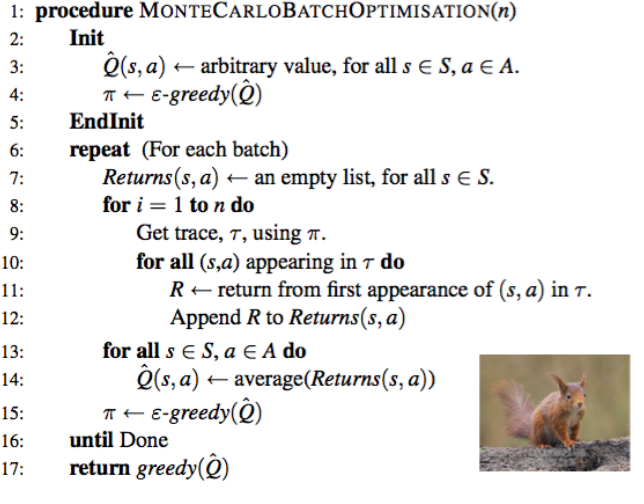
\includegraphics[scale=0.5]{figures/mc_batch_greedy.PNG}
%   \caption{MC Batch Learning to Control; Source: Lecture}
%   \label{fig:mc_batch_greedy}
% \end{figure}
% \begin{figure}[h!]
%   \centering
% %   \hspace*{-1cm}  
%   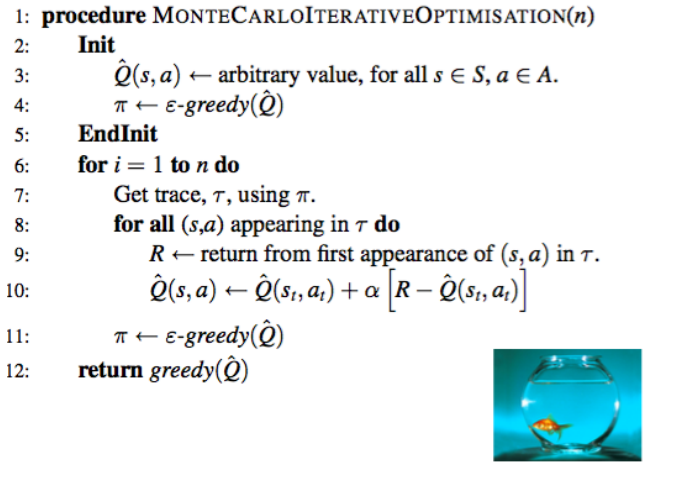
\includegraphics[scale=0.5]{figures/mc_iterative_greedy.PNG}
%   \caption{MC Iterative Learning to Control; Source: Lecture}
%   \label{fig:mc_iterative_greedy}
% \end{figure}

% \subsection{MC summary}
% one of the issues in MC is sufficient exploration of all available actions. In simulated environments this issues can be tackled with randomness for state-action values at the start of  the learning process but harder to arrange in learning from real experience. \\

% "In on-policy the agent commits to exploration and learns the respective stochastic policy while in off-policy an agent learns a deterministic policy separate from the one followed. Typically off-policy methods rely on some form of importance sampling."

\subsection{Temporal Difference Control -- SARSA}
Temporal Difference has several advantages over MC such as lower variance and online learning so we can combine the $\epsilon$-greedy policy improvement and TD update rule from equation \ref{eq:td_update} with Q(S,A) \cite{lecture_mfc} (basically replacing V with Q) :
\begin{align}
    Q(S, A) \longleftarrow Q(S, A) + \alpha (r + \gamma Q(S', A') - Q(S, A)) \label{eq:sarsa_update_rule}
\end{align}
% \begin{figure}[h!]
%   \centering
% %   \hspace*{-1cm}  
%   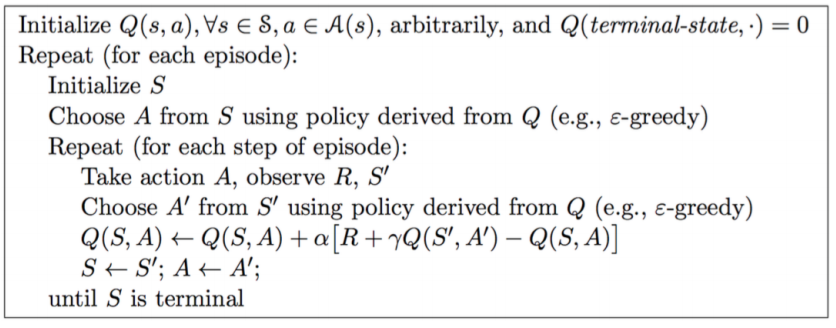
\includegraphics[scale=0.5]{figures/sarsa.PNG}
%   \caption{SARSA - On-Policy learning TD control; Source: \cite{lecture_mfc}}
%   \label{fig:sarsa}
% \end{figure}

This update rule forms the SARSA algorithm, deriving its name
from the typical transition an agent undergoes -- 
($S$, $A$, $R$, $S^'$, $A^'$)\\

\begin{algorithm}[H]
\SetAlgoLined
Arbitrarily initialize $Q(s, a), \forall s \in S, \forall a \in A$\;
initialize S arbitrarily\;
from S choose action A using the $\epsilon$-greedy policy\;
\While {$S$ is not $S_{terminal}$}{
take action A, observe R, S^{'}\; \\
from $S^{'}$ choose action $A^'$ using the $\epsilon$-greedy policy\;
Q(S, A) \longleftarrow Q(S, A) + \alpha (R + \gamma Q(S', A') - Q(S, A))\;\\
S \longleftarrow S^{'}\;\\
A \longleftarrow A^{'}\;\\
}
\caption{SARSA -- on-policy temporal difference learning. Source: \cite{lecture_mfc} }
\label{algorithm:sarsa}
\end{algorithm}\\

\\SARSA converges under the conditions of GLIE sequence of policies $\pi^k(a, s)$ and Robbins-Monroe sequence of step-sizes $\alpha_t$. So $\epsilon$ and $\alpha$ need to be adjusted over time \cite{lecture_mfc}.

% "One issue for SARSA is sparse rewards when the reward 
% propagates down a trace through many episodes slowly. Two ways to deal with it are SARSA-Lambda and Hindsight Experience Replay"

\subsection{Off-policy Q-learning}

As mentioned above in off-policy a different policy  $\pi'$ is used to generate the data while estimating and optimizing $Q^{\pi}$ and $V^{\pi}$ still. $\pi$ is the target policy and $\pi'$ is the  behaviour policy. An important assumption to ensure learning the assumption of coverage: $\pi(a, s) > 0 => \pi'(s, a) > 0$ \cite{lecture_mfc}.\\

% "One of the most important breakthroughs in reinforcement learning was the development of off-policy TD control algorithm known as Q-learning (Watkins, 1989)." [LECTURE]

In Q-learning the  next action is chosen using the behaviour policy, but in the update rule we use the alternative greedy successive action based on the target policy: $\max_a Q(s_{t+1}, a)$\\

In this way both the target and behaviour policies improve, target policy being greedy w.r.t. $Q(S, A)$ and behaviour policy being $\epsilon$-greedy w.r.t $Q(S, A)$. The Q learning target is then respectively: $r_{t+1} + \max_{a'} \gamma Q(s_{t+1}, a')$\\

% \begin{figure}[h!]
%   \centering
% %   \hspace*{-1cm}  
%   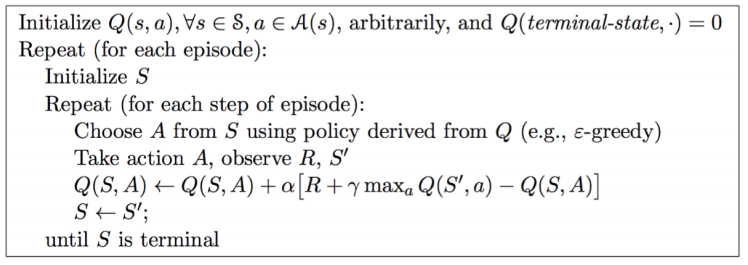
\includegraphics[scale=0.5]{figures/q_learning.PNG}
%   \caption{Q-Learning algorithm; Source: \cite{lecture_mfc}}
%   \label{fig:q_learning}
% \end{figure}

\begin{algorithm}[H]
\SetAlgoLined
Arbitrarily initialize $Q(s, a), \forall s \in S, \forall a \in A$\;
initialize S arbitrarily\;
\While {$S$ is not $S_{terminal}$}{
from S choose action A using the $\epsilon$-greedy policy\;
take action A, observe R, S^{'}\; \\
Q(S, A) \longleftarrow Q(S, A) + \alpha (R + \gamma \max_{a} Q(S', a) - Q(S, A))\;\\
S \longleftarrow S^{'}\;\\
}
\caption{Q-learning -- off-policy temporal difference learning. Source: \cite{lecture_mfc} }
\end{algorithm}\\


There are no explicit policies here: target policy is implicit in the greedy term $max_a Q(S', a)$ and behaviour policy is the $\epsilon$-greedy version of the target policy that we use to choose $A$. Both policies are updated with the update rule.

\subsection{Cliff walking  Q-learning vs. SARSA}
One very well known example demonstrating the difference between
Q-learning and SARSA or in other words Off-policy and On-policy learning methods was presented by Sutton and Barto \cite{sutton_barto}. They look at a case of an agent traversing a grid from left to right bypassing a cliff's edge as shown in the figure \ref{fig:cliff}. Each
step in the grid gives a reward of -1 and "falling off" 
the cliff results in a reward of -100 and the agent goes
back to the starting position.

\begin{figure}[H]
\centering
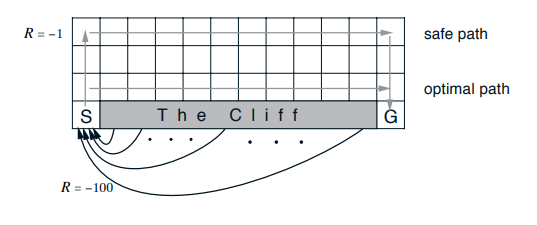
\includegraphics[scale=0.6]{figures/cliff_scheme.PNG}
  \caption{Cliff walking example; Source: \cite{sutton_barto}}
  \label{fig:cliff}
\end{figure}

Here Q-learning and SARSA produce different optimal policies. Q-learning gives the "optimal path" walking near the edge, while SARSA suggests a "safer path" further
from the cliffs edge and despite the former clearly 
being the preferred option Q-learning still performs 
worse than SARSA based on the overall reward score as can be seen from figure \ref{fig:cliff_score}

\begin{figure}[H]
\centering
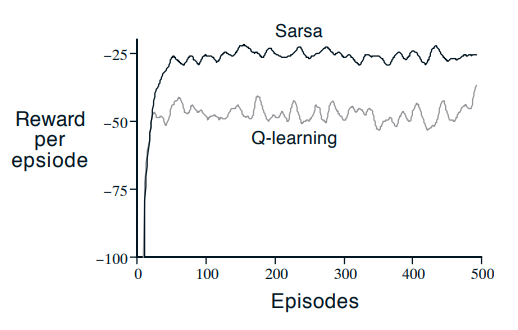
\includegraphics[scale=0.6]{figures/cliff_score.PNG}
  \caption{Cliff walking results; Source: \cite{sutton_barto}}
  \label{fig:cliff_score}
\end{figure}

As Sutton and Barto recognize \cite{sutton_barto} this 
arises precisely from the on and off policy nature of 
these 2 approaches. Q-learning still acts based on its
\textbf{behaviour policy} unrelated to the optimal target policy it optimizes and thus due to it being $\epsilon$-greedy when walking near the cliff it occasionally "falls off" and this affects the overall
reward score.  At the same time because SARSA is 
optimizing the same policy it follows it learns a safer
path further from the edge because it takes the \textbf{next} action selection into account. 
It follows the next selected action as can be seen from the 
algorithm \ref{algorithm:sarsa} and accounts for its Q value.

\section{Function Approximation}

\subsection{Limitations of tabular}

In Tabular Q learning due to the discrete nature of 
state and action spaces it is harder to represent the real world accurately as the problem of fine discretisation arises: the approximation needs to be accurate enough for meaningful learning. But this can be memory inefficient as the number of parameters grows \cite{lecture_intro_to_deep_rl}. \\

Another important limitation affects the exploration ability of the learning agent: each Q entry for subsequent state-action entries need to be updated independently despite obvious correlation between them.\\

One solution to this is function approximation.

\section{Deep learning}

A neural network consists of multiple layers of interconnected neurons each defined by a weight and bias that are applied to the incoming signal \cite{lecture_intro_to_deep_rl}.\\

In supervised learning there's usually a reference that 
the network is trained against, for example in classification the reference might be a label to an RGB image. The model then learns weights such that the desired outputs are produced on respective inputs \cite{lecture_intro_to_deep_rl} . \\

This is achieved through backpropagation and gradient descent where the difference between current weights and desired weights is evaluated using a cost functions and applied until convergence \cite{lecture_intro_to_deep_rl} .\\

For example for a dataset with $x_i$ input paired with a $y_i$ label cost function would be: 
\begin{align}
    C(\theta, D) = [y_i - f(x_i)]^2
\end{align}

\section{Deep Q learning}

So our goal now is to approximate the Q-table with a neural network that accepts state and outputs Q(s, a) 
values for the whole range of actions \cite{lecture_intro_to_deep_rl}. Thus we make state space continuous, while action space is still discrete, like in figure \ref{fig:q_network  }.

\begin{figure}[H]
  \centering
%   \hspace*{-1cm}  
  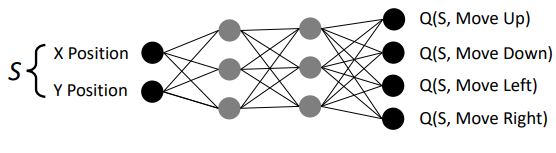
\includegraphics[scale=0.5]{figures/q_network.PNG}
  \caption{Example Q network for traversing a 2D space; Source: \cite{lecture_intro_to_deep_rl}}
  \label{fig:q_network  }
\end{figure}

Adapting the Temporal Difference Error term from the TD update rule \ref{eq:td_update} into the context of neural network cost function we get \cite{lecture_intro_to_deep_rl}:
\begin{align}
    C(\theta, D) = [R + \gamma \max_a Q(S', a) - Q(S, A)]^2
\end{align}
% \begin{figure}[h!]
%   \centering
% %   \hspace*{-1cm}  
%   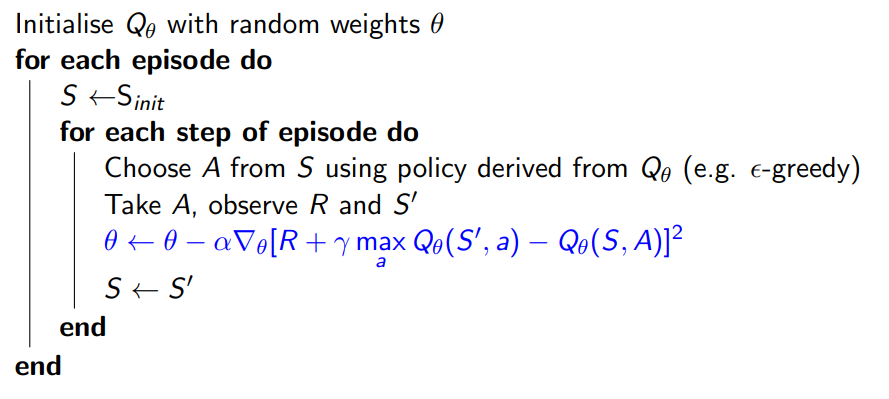
\includegraphics[scale=0.5]{figures/dqn_first.PNG}
%   \caption{Deep Q-learning algorithm; Source: \cite{lecture_dqn}}
%   \label{fig:dqn_first}
% \end{figure}

\begin{algorithm}[H]
\SetAlgoLined
Initialize $Q_{\theta}$ with random weights \theta \; \\
initialize S arbitrarily\;\\
\While {$S$ is not $S_{terminal}$}{
from S choose action A using the $\epsilon$-greedy policy\;
take action A, observe R, S^{'}\; \\
\theta \longleftarrow \theta - \alpha \nabla_{\theta}[R + \gamma \max_{a} Q_{\theta}(S', a) - Q(S, A)]^{2}\;\\
S \longleftarrow S^{'}\;\\
}
\caption{Deep Q-learning. Source: \cite{lecture_dqn} }
\end{algorithm}\\

\subsection{Overfitting}
% Like any neural network it can overfit but the random starts nature of LR counteracts that in effect [QnA]

\section{Experience Replay Buffer}

One limitation of online learning is that one transition needs to be visited many times for the network to learn appropriate weights ("many updates per transition" \cite{lecture_dqn}). \\

A solution is to create a dataset of all the experienced data so far collected by the agent. The advantage is that any transition can be sampled from the replay buffer and trained on more than once \cite{lecture_dqn}. 

\subsection{Mini batch learning }

Another limitation of deep Q-learning is that since now Q is represented not by a table, but by a continous function, neighbouring state values will affect each other easily due to correlation between them \cite{lecture_dqn} . And if 
we update the function in a consecutive manner (going by consecutive states in the order they were collected for example) this will cause the  Q-distribution to start changing rapidly and affect the untrained parts of the Q-network and cause uneven learning \cite{lecture_dqn}. \\

One solution is to sample transitions from the replay buffer not in the order they were collected but in random mini-batches\cite{lecture_dqn}. This causes a more uniform, even learning and update of the Q function \cite{lecture_dqn}.  

% \begin{figure}[H]
%   \centering
% %   \hspace*{-1cm}  
%   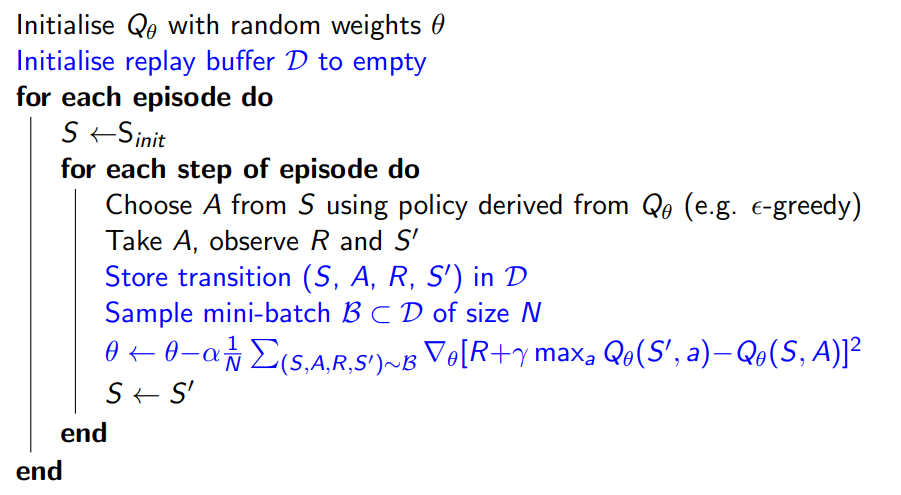
\includegraphics[scale=0.5]{figures/replay_buffer.PNG}
%   \caption{Deep Q -learning algorithm with replay buffer; Source:\cite{lecture_dqn}}
%   \label{fig:replay_buffer}
% \end{figure}

\subsection{Prioritised Experience Replay}

On top of sampling transitions in minibatches in a uniform random manner it may be useful to note that some transitions might be more important than others and sampling them more frequently may boost the learning process. \cite{lecture_dqn}. Hence the idea of prioritised experience replay buffer. \\

A way to tell which transitions are more important than others is to see the magnitude of the prediction error $\delta = R + \gamma \max_a Q_{\theta}(S', a) - Q_{\theta}(S, A)$. 
Intuitively greater error results in greater learning.\\

So each transition is assigned a weight $w_i = |\delta| + \epsilon$, where $\epsilon$ is a small constant ensuring each transition has a probability of being sampled greater than 0. Thus the sampling probability for a transition $i$ is:
\begin{align}
    p_i = \frac{w_i^{\alpha}}{\sum_k w^{\alpha}_k}
\end{align}

Where $\alpha$ determines how much individual transitions are prioritized over the others with $\alpha = 0$ being equivalent to uniform sampling.\\

It only makes sense to update only the weights for transitions that were sampled, since we already have their $\delta$ error values\cite{lecture_dqn}. For new transitions pushed to the replay buffer, assign the current maximum weight to ensure that they can be sampled and that sufficient exploration is done.

% \begin{figure}[H]
%   \centering
% %   \hspace*{-1cm}  
%   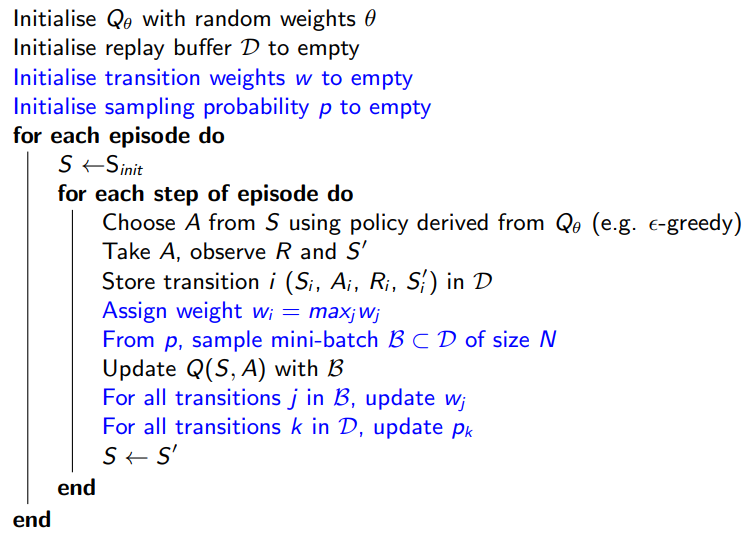
\includegraphics[scale=0.5]{figures/prioritized_buffer.PNG}
%   \caption{Prioritised Experience Replay Algorithm; Source: \cite{lecture_dqn}}
%   \label{fig:replay_buffer}
% \end{figure}

\section{Target Network }

As we have seen before with mini-batch sampling having an approximated Q function introduces certain challenges. 
For example when adjacent states are trained on multiple times
it results in a rocketing effect with the Q function basically "chasing its own tail" in a sense \cite{lecture_dqn}.  
\begin{figure}[h!h!h!h]
\centering
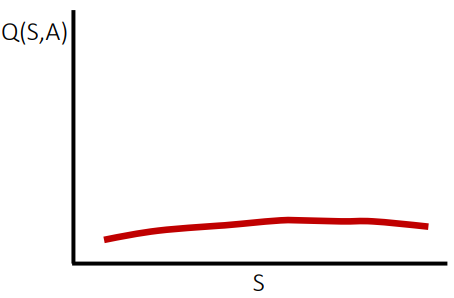
\includegraphics[scale=0.5]{figures/target 1.PNG}
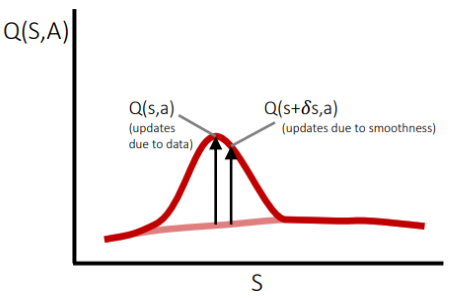
\includegraphics[scale=0.5]{figures/target 2.PNG}\\
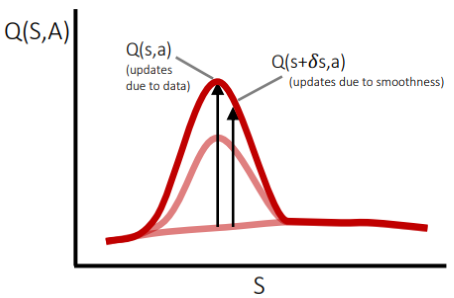
\includegraphics[scale=0.5]{figures/target 3.PNG}
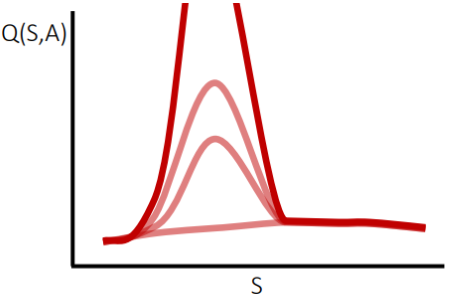
\includegraphics[scale=0.5]{figures/target 4.PNG}
  \caption{Generalisation effect on learning; Source: \cite{lecture_dqn}}
  \label{fig:generalisation_curse}
\end{figure}

This correlation between adjacent states can be tracked down to the $\max_a Q_{\theta}(S', a)$ term in the update step. Hence the 
extension to DQN is to introduce a separate Target Network $\hat{Q}$ to calculate the prediction error. This allows Q network to learn independently from the generalisation effect \cite{lecture_dqn}. Every now and then $\hat{Q}$ is set to Q.

\begin{figure}[H]
\centering
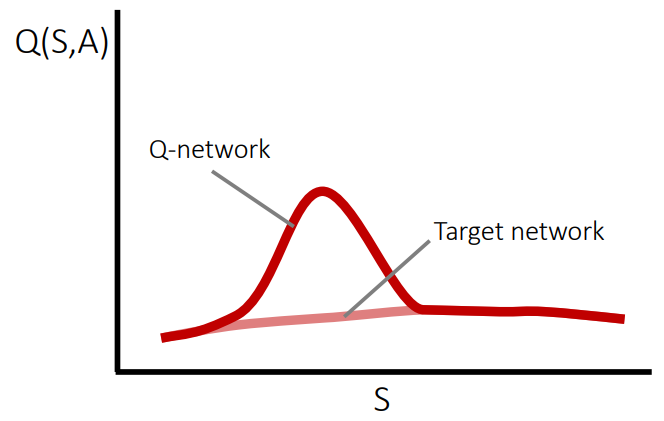
\includegraphics[scale=0.4]{figures/target 0.PNG}
  \caption{Target network; Source: \cite{lecture_dqn}}
  \label{fig:target_network}
\end{figure}

Here's the updated algorithm for Deep Q-learning with target network extension.

% \begin{figure}[H]
% \centering
% 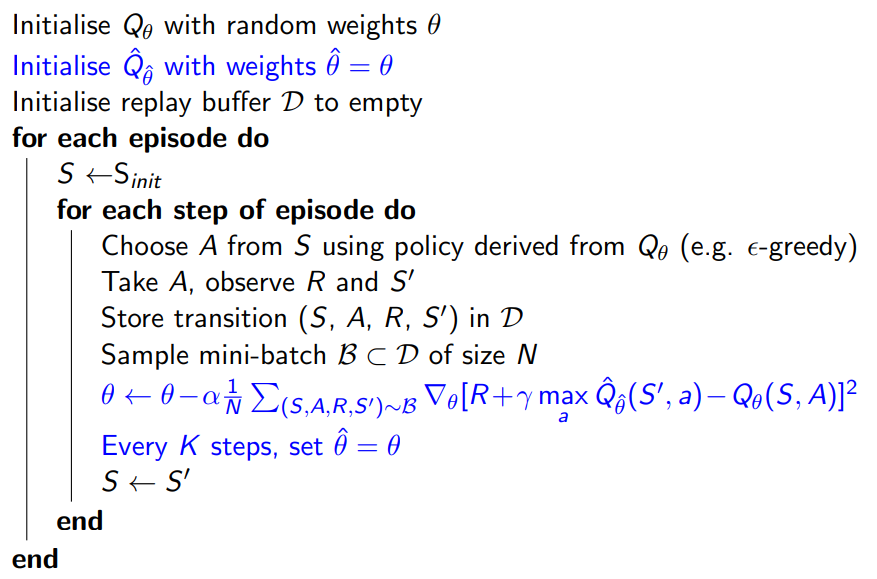
\includegraphics[scale=0.4]{figures/dqn wth target.PNG}
% % \caption{The Universe}
%   \caption{Deep Q-Learning with Target Network; Source: Lecture}
%   \label{fig:target_network_algorithm}
% \end{figure}

\section{Double Deep Q-learning}
Another issue that still arises is the problem of overestimation when picking the greedy action in the target $R + \gamma \max_a \hat{Q}_{\hat{\theta}}(S' a)$. Target network is a noisy estimation for different action values (for an arbitraty state) and the sampled maximum $\hat{Q}$ value might not be the maximum for the true $Q$ function for the same action \cite{lecture_dqn}. In order to tackle this problem of overestimation 
further decoupling is introduced in the target term.\\

In Double Deep Q-learning different networks are used to pick the maximum action and estimate its Q value. This on average reduces the amount by which an action is overestimated since an unusually high value in one network is unlikely to be such in the other \cite{lecture_dqn}. Thus the new error in the update step in the algorithm is either:
\begin{align}
    [R + \gamma Q_{\theta}(S', \text{arg}\max_a\ \hat{Q}_{\hat{\theta}}(S', a)) - Q_{\theta}(S, A)]^2
\end{align}
or:
\begin{align}
    [R + \gamma \hat{Q}_{\hat{\theta}}(S', \text{arg}\max_a\ Q_{\theta}(S', a)) - Q_{\theta}(S, A)]^2
\end{align}

\begin{algorithm}[H]
\SetAlgoLined
Initialize $Q_{\theta}$ with random weights \theta \; \\
Initialize $\hat{Q}_{\hat{\theta}}$ with weights \theta \; \\
Initialize replay buffer $B$\; \\
initialize S arbitrarily\;\\
\While {$S$ is not $S_{terminal}$}{
from S choose action A using the $\epsilon$-greedy policy\;
take action $A$, observe $R$, $S^{'}$\; \\
store transition ($S$, $A$, $R$, $S^{'}$) in B\; \\
sample min-batch D $\subset$ B of size N\; \\
\theta \longleftarrow \theta - \alpha \frac{1}{N} $\sum_{(S,A,R,S^{'}) \sim B} \nabla_{\theta}[R + \gamma Q_{\theta}(S', \text{arg}\max_a\ \hat{Q}_{\hat{\theta}}(S', a)) - Q_{\theta}(S, A)]^{2}$\;\\
Every K steps, $\hat{\theta} = \theta$ \;\\
S \longleftarrow S^{'}\;\\
}
\caption{Double Deep Q-learning with Prioritised Replay Buffer. Source: \cite{lecture_dqn} }
\end{algorithm}\\



% \subsection{3 network architectures}
% \subsection{REINFORCE ALGORITHM}
% \subsection{deterministic vs stsochastic policies}
% \subsection{reducing variance}
% \subsection{model free vs model based}
% \subsection{planning in discrete spaces (irrelevant to LoRa) }
% \subsection{Cross Entropy }
% \subsection{method for continuous spaces (relevant?)}
% \subsection{model predictive control}

\chapter{Learning Model}
\section{Distributed Learning}

The ideal situation would of course be having one learning agent 
per LoRa node so they could learn a policy specifically suited for
that one node. But the case is that typically nodes located 
near each other can benefit from one policy [CITATION or EXPERIMENT]
so in order not to waste memory on slightly different models 
for nodes located near each other nodes can be grouped into clusters
and share learning weights.



Despite first prototypes starting with 

\section{LoRa State}
\section{LoRa Action}
\section{LoRa Reward}

\section{SINR}
The \texttt{SINR Model} is implemented similarly to how \texttt{SNR Model} was implemented in the original simulator \cite{simulator}. The model calculates signal-to-interference noise ratio (SINR) for the received signal strength values of packets in the air according to this formula [CITE WIKIPEDIA???]:
\begin{align}
    \text{SINR}(x) = \frac{P}{I + N} \label{eq:sinr}
\end{align}
where:
\begin{align*}
     P &- \text{power of the examined signal}\\
     I &- \text{total interference from weaker signals in the air}\\
     N &- \text{ noise floor}\\
\end{align*}

The interference is only calculated from the weaker signals, since we're assuming that NOMA is enabled at 
the gateway and thus all the stronger signals would be
decoded apriori \cite{noma_original}.\\

\texttt{SINR Model} also calculates throughput from SINR values. The need for throughput metric will be explained below. This formula [CITE WIKI???] is used:

\begin{align}
    \text{throughput} = \text{$log_{2}$}(\text{sinr} + 1)
\end{align}

\chapter{Evaluation Plan}
% "Evaluation plan (1-2 pages). Project evaluation is very important, so it's important to think now about how you plan to measure success. For example, what functionality do you need to demonstrate?  What experiments to you need to undertake and what outcome(s) would constitute success?  What benchmarks should you use? How has your project extended the state of the art?  How do you measure qualitative aspects, such as ease of use?  These are the sort of questions that your project evaluation should address; this section should outline your plan."

The ultimate end goal of the project would be training an RL deep neural network model algorithm that would outperform the existing Adaptive Data Rate (ADR) mechanism for optimizing data rates, airtime and energy consumption in a LoRaWAN network.\\

The most relevant aspects of LoRaWAN communication to us are Energy efficiency and Data Extraction Rate over a noisy channel. The final evaluation would involve conducting experiments with the simulator described above running 2 algorithms against each other.

%https://ieeexplore.ieee.org/stamp/stamp.jsp?tp=&arnumber=8406255
\chapter{Ethical issues}
%"Ethical issues (1-2 pages). What are the wider ethical, legal, professional and societal issues surrounding your project and the accompanying research? You should use the ethics checklist as the basis for this discussion. "

Since the project mostly involves working with relatively low level embedded software for resource management optimization the immediate ethical implications are quite vague and non obvious. \\

Looking at IoT applications as a whole of course they touch a multitude of areas and industries including Agriculture, Oil\&Gas and Military \cite{lora_battlefield} \cite{lora_troops} each of which involves various ethical issues such as environmental issues, animal abuse and human rights.
% \appendix
% \chapter{First Appendix}


\bibliographystyle{unsrtnat}
\bibliography{bibs/sample}

\end{document}